\subsection{What is Spectral Analysis?}
So far we've been studying time series $\{X_t\}_{t\in \mathbb{Z}}$, with models of the form \[X_t=\mu_t +\sum_{j=0}^\infty \Psi_j \epsilon_{t-j} \]
We have seen, this encompasses the usual SARIMA processes (by writing the AR parts as MA($\infty$)). However, this applies also to any weakly stationary time series \footnote{This is the statement of Wold decomposition theorem.}. We have seen that we can decompose time series into trend, cycle and noise components. All of our analyses, e.g. calculation of covariances and correlations between different dates, was based on this representation. This type of analysis, i.e. decomposing a time series into elements across different time periods, is known as \textbf{time domain} analysis.\\

However, this is not the only way of interpreting time series data. If we are primarily concerned in analyzing periodicities in our data, i.e. in economic terms different levels of seasonality, then the perspective of \textbf{frequency domain} or \textbf{spectral analysis} becomes useful. This involves decomposing a time series into an overlay of different periodic functions (i.e. sine and cosine) at different frequencies (meaning, a bit simplified, we find the linear combination of sine and cosine functions at different frequencies that reproduce our time series) and calculating how much of our process' total variance is due to individual frequencies.\\

\noindent
\rule{\linewidth}{0.4pt}

\subsubsection{Class example}

\begin{figure}[h]
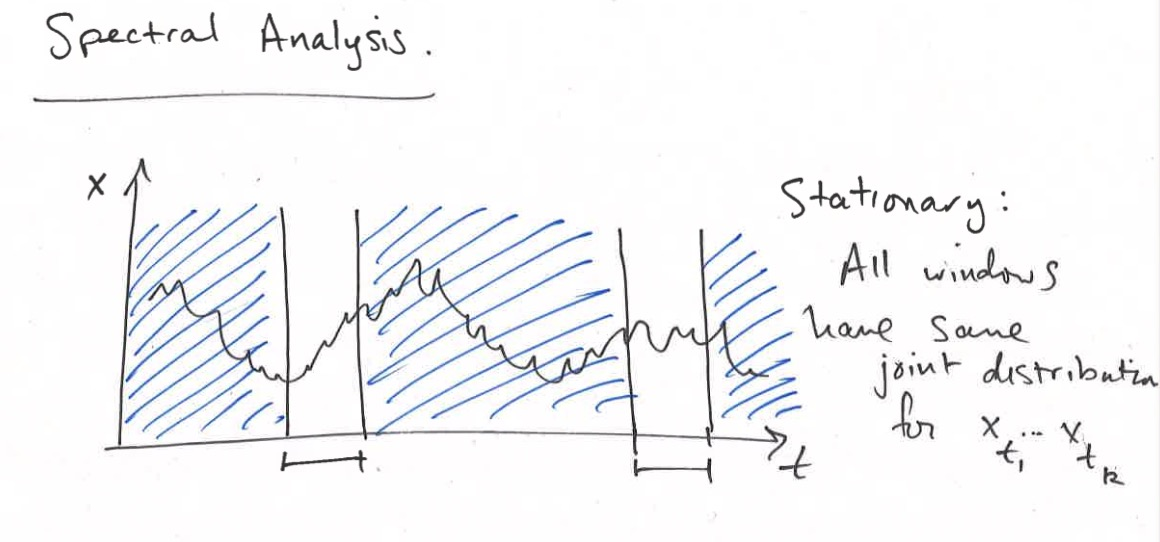
\includegraphics[scale=0.3]{images/Screenshot 2024-04-29 at 08.36.41.jpg}
\centering
\end{figure}


\underline{Question:} Is the following time series stationary:\\
    \[X_t = R \cdot \cos(t+ \phi) + \varepsilon_t\] 
\begin{itemize}
    \item[] Let $R>0$ be a positive random variable.
    \item[] Let $\phi \in [0, 2\pi]$ be a uniform random variable
    \item[] Let $\varepsilon_t$ $t \in Z$ (so $t=...,-2-1,0,1,2,...$)
    \item[*] \underline{Answer}: It is stationary: Why? 
    \begin{itemize}
        \item[] Compare to $W_t = \cos(t)+ \varepsilon_t$ (i.e., $R=1, \phi = 0$ instead of random) $\Rightarrow$ Not-stationary 
    \end{itemize}
\end{itemize}

\begin{figure}[H]
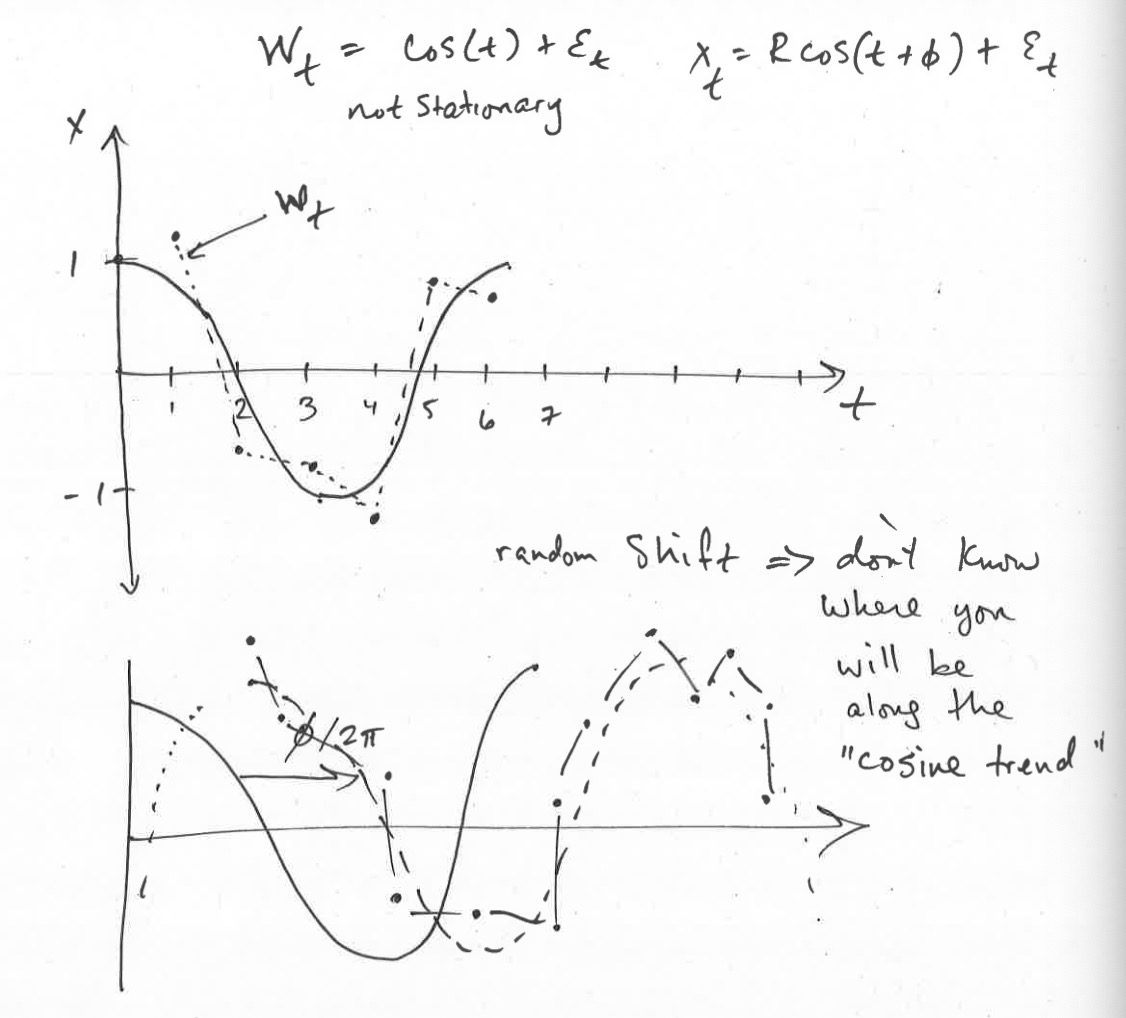
\includegraphics[scale=0.25]{images/Screenshot 2024-04-29 at 08.38.34.jpg}
\centering
\end{figure}

\begin{figure}[h]
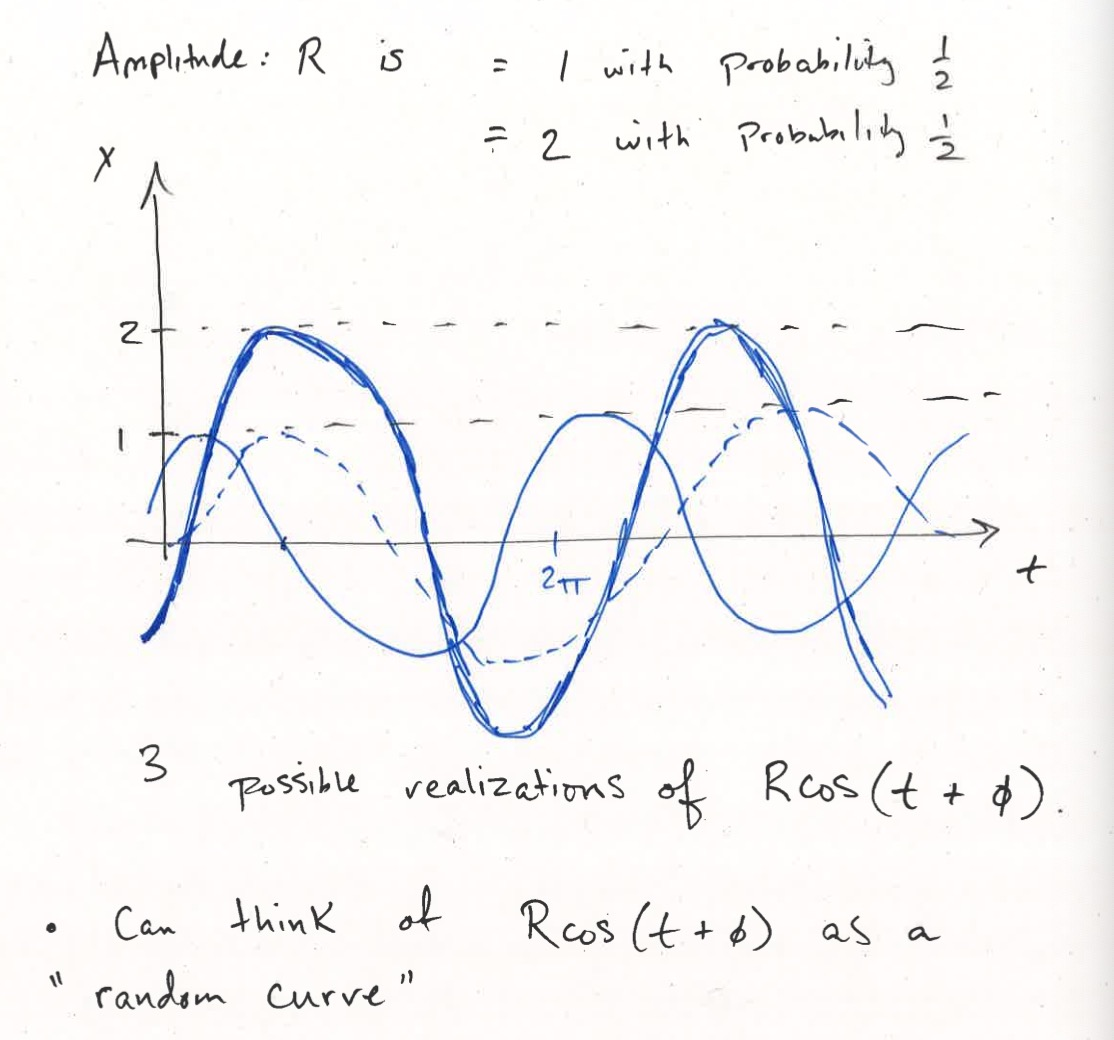
\includegraphics[scale=0.25]{images/Screenshot 2024-04-29 at 08.38.59.jpg}
\centering
\end{figure}

\underline{Question:} Can all stationary time series be decomposed into a sequence of random curves of the form $R(\cos(wt + \phi))$ ? 

\[X_t = \sum_{j=1}^k R_j \cos(w_j t +\phi_j)+Z_t \]
with $w_j$ deterministic frequencies and $R_j, \phi_j$ random amplitudes and phases and $Z_t$ idiosyncratic or iid. 

\underline{Answer:} In a certain sense, yes: \
But have to let $k\rightarrow \infty$ and take a limit in the right way. \\

\noindent
\rule{\linewidth}{0.4pt}
\bigskip

For spectral analysis, we again start with a stationary process $\{X_t\}_{t\in \mathbb{Z}}$ and write it in the form 
\begin{align}
    X_t=\mu+\int_0^\infty \left[\alpha(\omega) \cos(\omega t) + \delta(\omega) \sin(\omega t) \right] d\omega, \quad \forall t \in \mathbb{Z} \label{SP1}
\end{align}


A priori, it is not obvious that such decomposition (\ref{SP1}) always exists. The \textbf{spectral representation theorem} however answers this in the affirmative. How can sine and cosine functions (which have a very rigid periodic structure) reconstruct a function (i.e. the time series) that does not (necessarily) have the same regular periodic structure? For intuition, we illustrate this phenomenon using the (scaled) Gaussian kernel function: \[f(x)=\frac{1}{\sqrt{2\pi}}e^{-\frac{x^2}{2}} \]
We want to approximate this function using sine and cosine functions. Recalling that we can write $e^{i\omega j} = \cos(\omega j) + i \sin(\omega j)$, we want to write \[f(x) \approx \frac{1}{N} \sum_{j=0}^{N-1}a_j e^{i2\pi\frac{1}{N} x} \] i.e. as a linear combination of N periodic functions of different frequency. Finding the appropriate weights $a_j$ is called calculating the \textbf{Fourier transform} of $f$. One can show that for $N\rightarrow\infty$, one is able to perfectly reproduce $f$\footnote{More precisely, $\sin(\pi n x)$ and $\cos(\pi nx)$ for $n \in \mathbb{N}$ form a basis for the space of square integrable functions}; for $N$ finite, there will be an approximation error. As $N$ increases, the approximation error decreases: 

\begin{figure}[h]
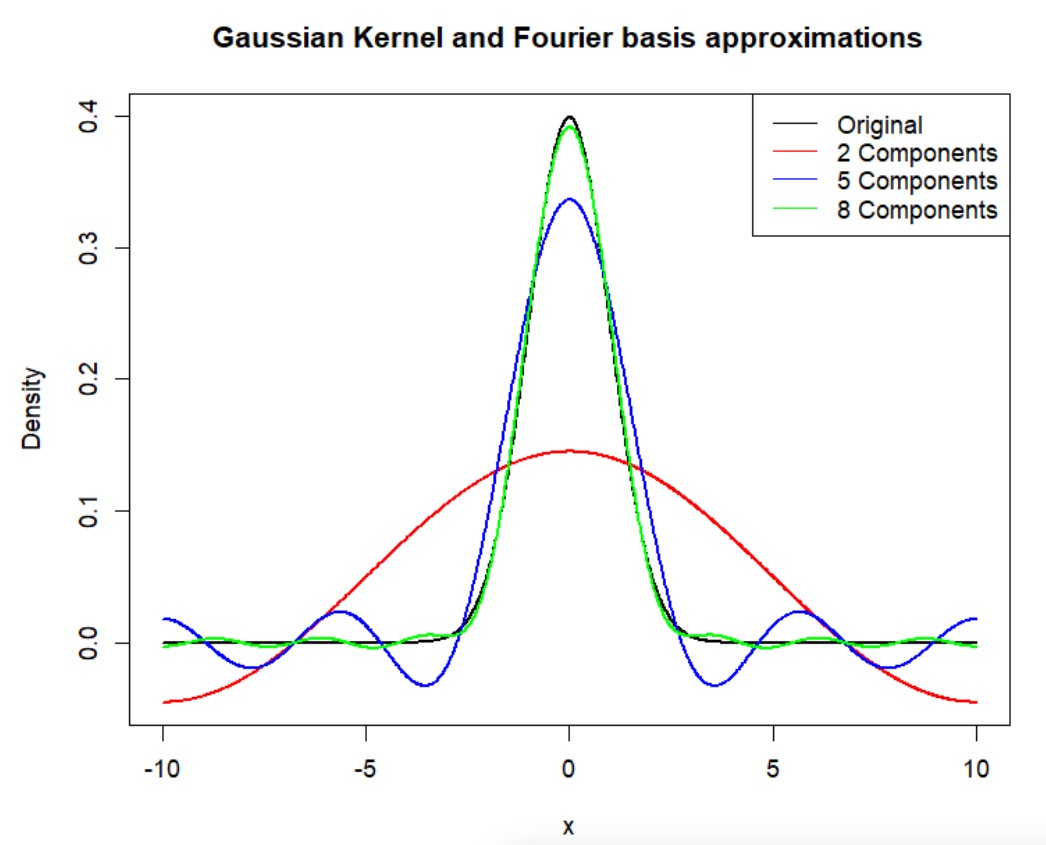
\includegraphics[scale=0.3]{images/Screenshot 2024-05-06 at 09.35.47.jpg}
\centering
\caption{Successive approximation of the gaussian kernel using a Fourier basis. The global approximation error decreases as we increase the number of basis functions}
\end{figure}

How does this relate to time series? Any time series $\{X_t\}_{t\in \mathbb{Z}}$
 can be interpreted as points subsampled from a continuous curve $\{X_t\}_{t\in \mathbb{R}}$. It is possible to define the Fourier transform for both functions on $\mathbb{R}$ (i.e. with uncountable support) and for discrete series (e.g. deterministic time series), simply by exchanging summation and integration. The interpretation of these operations is similar.\\

 Modelling time series differs from function approximation (as above) in that randomness is involved. Hence, rigorously speaking, one cannot apply the above considerations directly to $\{X_t\}_{t\in \mathbb{Z}}$. The appropriate generalization of the Fourier decompositions to random series is the already mentioned spectral representation theorem, stating that any weakly stationary time series can be written as \[X_t=\mu+\int_0^\infty \left[\alpha(\omega) \cos(\omega t) + \delta(\omega) \sin(\omega t) \right] d\omega, \quad \forall t \in \mathbb{Z}\]
 Here, the \textbf{"coefficient functions"} $\alpha(\cdot)$ \textbf{and} $\delta(\cdot)$ \textbf{are random} with the property that, for any frequencies $0<\omega_1<\omega_2<\omega_3<\omega_4<\pi$, the random variables $\int_{\omega_1}^{\omega_2}\alpha(\omega) d \omega $ and $\int_{\omega_3}^{\omega_4}\alpha(\omega) d \omega $, as well as $\int_{\omega_1}^{\omega_2}\delta(\omega) d \omega $ and $\int_{\omega_3}^{\omega_4}\delta(\omega) d \omega $ are uncorrelated. Also, $\alpha$ and $\delta$ are uncorrelated. So, instead of decomposing the process into random independent components at different times, we decompose it into (somewhat) independent components of different frequencies!

\subsection{Key Concepts}
Recall again the definition of the autocovariance function of a stationary process: \[
\gamma(k):=\mathbb{E}[(X_t-\mu)(X_{t-k}-\mu)] \quad \forall k\in \mathbb{N}
\]
We can apply the (discrete) Fourier transform operator to this (discrete) function: \[
f(\omega):=\frac{1}{2\pi} \sum_{j=-\infty}^\infty \gamma(j) e^{-i\omega j}
\] \

because $e^{-i\omega k} = \cos(\omega k) + i \sin(\omega k)$ and $\gamma(k) = \gamma(-k)$ so the "$\sin$" terms cancel out. \\



This new function $f(\cdot)$ is called the \textbf{spectral density} or \textbf{spectrum} of $\{X_t\}_{t\in \mathbb{Z}}$. Since $\gamma(k)=\gamma(-k)$, and using some basic properties of the sine and cosine functions, the spectral density simplifies to: \[
f(\omega)=\frac{1}{2\pi}\{\gamma(0) + 2\sum_{j=1}^\infty \gamma(j) \cos(\omega j)\}
\]

\textbf{Example 1.} The spectrum for:
\begin{enumerate}
    \item White noise: \[
    f(\omega) = \frac{\sigma_Z^2}{\pi}
    \]
    \item MA(1): \[
    f(\omega)=\frac{1}{\pi}(1+\theta^2+2\theta\cos(\omega))\sigma_Z^2
    \]
    \item for ARMA(p,q), i.e. $X_t=\mu+\phi_1 X_{t-1}+\cdots+\phi_p X_{t-p} + \epsilon_t + \theta_1 \epsilon_{t-1} + \cdots +\theta_q \epsilon_{t-q} $, one can show that \[
    f(\omega)=\frac{\sigma_Z^2 \prod_(j=1)^q(1+\eta_j^2-2\eta_j \cos(\omega)) }{2\pi \prod_{j=1}^p(1+\lambda_j^2-2\lambda_j\cos(\omega)) }
    \] where $\eta_j$ and $\lambda_j$ are the inverted roots of the characteristic polynomials of the MA and AR parts, respectively.
\end{enumerate}

We have defined the spectral density as a function of the autocorrelations, i.e. the latter implying the former. Actually, both are equivalent, meaning that one can also back out again the autocorrelations from the spectral density: \[
\gamma(k)=\int_{-\pi}^\pi f(\omega) e^{i\omega k} d\omega
\]
This mathematical fact is known in Analysis as the Fourier inverse \footnote{More precisely, for a given function $g$, we can define its Fourier transform $\hat{g}$ as \[
\hat{g}=\frac{1}{2\pi} \int_{-\infty}^\infty g(x)e^{-ix\omega} dx
\] The Fourier inverse theorem states that the converse is also possible: \[
g(x) = \int_{-\pi}^\pi \hat{g}(\omega)e^{ix\omega}d\omega
\]
}. Note that this implies:\[
\gamma(0) = \int_{-\pi}^\pi f(\omega) d\omega
\]
i.e. the variance of the process equals the integral of the spectrum on $[-\pi,\pi]$. Put differently, one can explain the total variance of the process using the information provided by the full spectrum. Actually, \textbf{this result generalizes in a useful way}: the \textbf{part of the variance that is due to frequencies less than} $\omega_1$ equals \[
\int_{-\omega_1}^{\omega_1}f(\omega)d\omega=2\int_0^{\omega_1} f(\omega)d\omega \label{SP2}
\] where the equality comes from the fact that $f(\omega)=f(-\omega)$

\bigskip
\textbf{Example 2.} Let us illustrate what this means in a toy example: consider the process defined as \[
X_t=\sum_{j=1}^M [\alpha_j \cos(\omega_j t) + \delta_j \sin(\omega_j t)]
\] i.e. a discretized version of (\ref{SP1}), using only a finite number of frequencies $0<\omega_1<\cdots<\omega_M<\pi$. The sequences $\{\alpha_j\}_{j=1}^M, \{\delta_j\}_{j=1}^M$ are assumed to be serially uncorrelated and mutually independent with $Var(\alpha_j)=Var(\delta_j)=\sigma_j^2$. Then:\footnote{Recall that $\sin^2(x)+\cos^2(x)=1$} \[
Var(X_t(=\sum_{j=1}^M \sigma_j^2 [\cos^2(\omega_j t)+ \sin^2 (\omega_j t)]=\sum_{j=1}^M \sigma_j^2
\] Hence the part of total variance due to cycles of frequencies less than or equal to $\omega_j$ is $\sum_{j=1}^i \sigma_j^2$ \
How do we use this? Due to (\ref{SP2}), we know that the portion of variance attributable to frequencies in $[\omega_1, \omega_2]$ is given by $2\int_{\omega_1}^{\omega_2}f(\omega)d\omega $. This mean that the area under the graph $f(\cdot)$ between $\omega_1$ and $\omega_2$ is indicative of the importance of the corresponding frequencies for the process overall. If this area is large, then a lot of variance is generated by these frequencies, indicating some seasonality in that area.\\

How do we estimate this? Directly estimating $\gamma(\cdot)$ for all periods and plugging it into $\frac{1}{2\pi}\sum_{j=-\infty}^\infty \gamma(j)e^{-i\omega j} $ is not possible, as we only have finitely many observations. Even the truncated version, i.e. \[ 
\hat{f}:=\frac{1}{2\pi}[ \hat{\gamma}(0)+2\sum_{j=1}^{T-1} \hat{\gamma}(j)\cos(\omega j) ]
\] is impractical, as we need to estimate just as many parameters as we have observations. One could truncate this series to include fewer terms (a fixed number $M$). Alternatively, one could estimate the parameters of the underlying process in the time domain (i.e. ARMA model estimation), and calculate the implied covariances. Other methods include the smoothed periodogramm and kernel-based methods.

\subsection{Application}

We apply this methodology to US manufacturing data, using the FED's monthly seasonally unadjusted monthly index of production. We calculate the spectrum of the raw series: 

\begin{figure}[H]
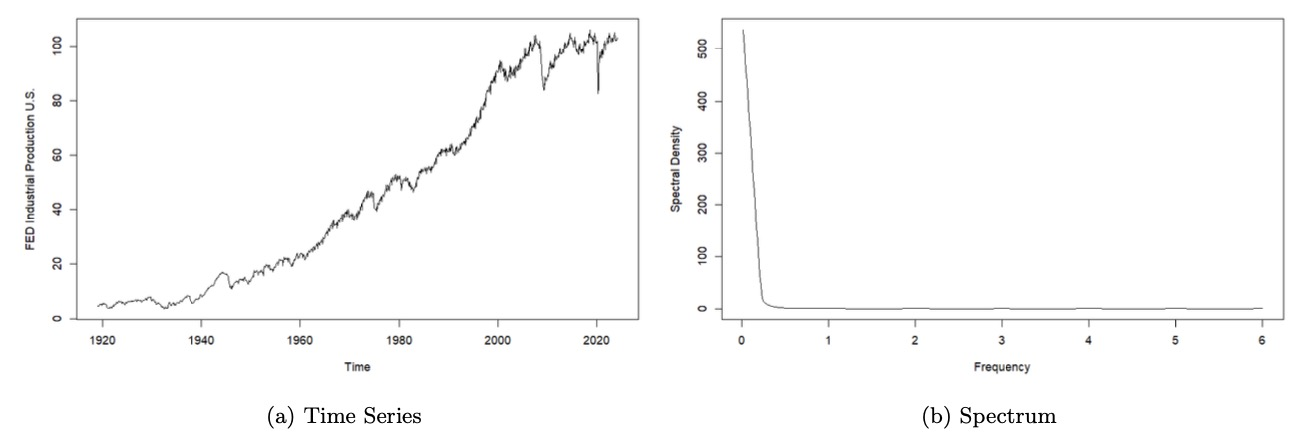
\includegraphics[scale=0.4]{images/Screenshot 2024-05-06 at 10.37.34.jpg}
\centering
\end{figure}

This does not yield meaningful results, as the method requires a stationary time series. In this case, the low-frequency (i.e. long-term) cycles induced by the uptrend dominate everything else. We therefore re-apply this method to the ime series of log-differences: 

\begin{figure}[H]
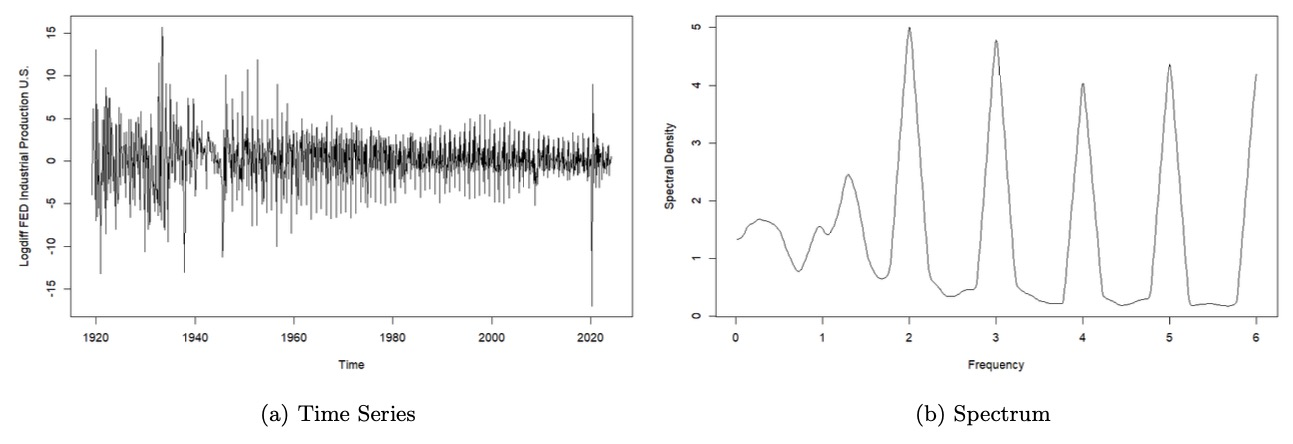
\includegraphics[scale=0.4]{images/Screenshot 2024-05-06 at 10.39.09.jpg}
\centering
\end{figure}

This gives an interpretable spectral density. Recall that the area under the curve represents the portion of total variance due to these frequencies. A spike at a certain frequency therefore means that it is important to the time series. In our case, we observe several spikes in the low frequencies (first and second bump), corresponding roughly to the business cycle (2.5 - 3 years) and a 12-month cycle. The remaining higher frequencies could potentially come from intra-year seasonalities, e.g. calendar effects. If we consider a year-on-year difference (log), then virtually all the seasonal components vanish, with only the business cycle frequency remaining: 
\begin{figure}[H]
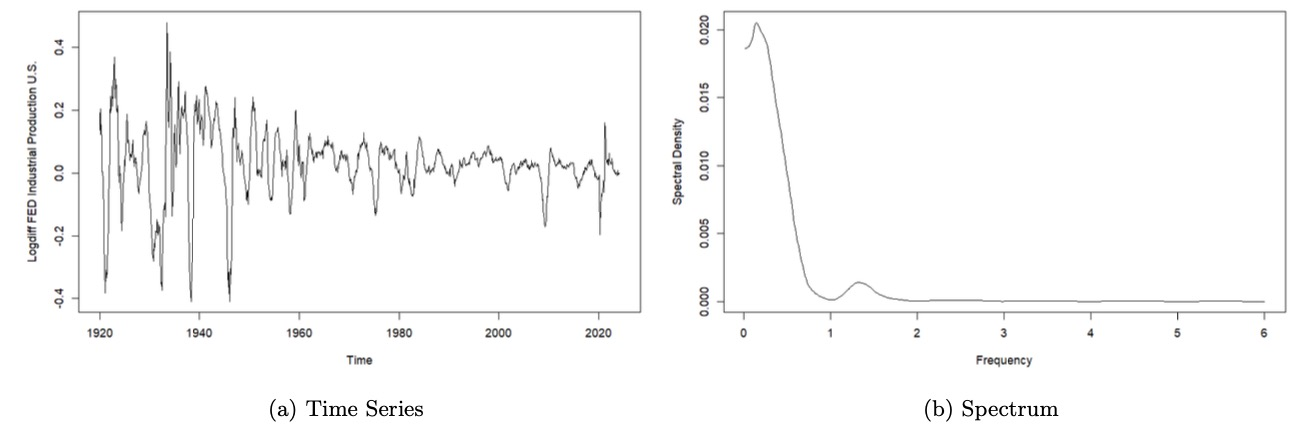
\includegraphics[scale=0.4]{images/Screenshot 2024-05-06 at 10.41.41.jpg}
\centering
\end{figure}




\subsection{Spectrum Calculation for White Noise Process}
\begin{align*}
    f(\omega)&=\frac{1}{\pi} \sum_{k=-\infty}^\infty \gamma(k) e^{-i\omega k}\\
    \gamma(0) & \neq 0 \quad \text{but $\gamma_k = 0$ \quad $\forall k\neq0$} \\
    &+ \frac{1}{\pi} \sum_{k\neq 0} \underbrace{\gamma(k)}_{=0} e^{-i\omega k} \\
    &= \frac{1}{\pi} \gamma(0)\\
    &= \frac{1}{\pi}var(X_t)
\end{align*}

\begin{figure}[H]
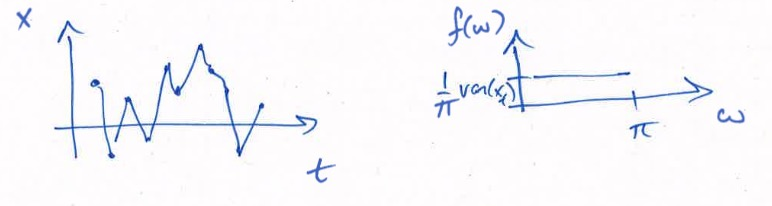
\includegraphics[scale=0.4]{images/Screenshot 2024-04-29 at 08.42.56.jpg}
\centering
\end{figure}



\subsection{Spectrum Calculation for MA process}
\[X_t=\varepsilon_t + \theta \varepsilon_{t-1}\]
what is $\gamma(k)$?
\begin{align*}
    \gamma(1)&=cov(\varepsilon_t+\theta \varepsilon_{t-1}, \varepsilon_{t-1} \theta \varepsilon_{t-2} \\
    &= cov(X_t, _{t-1})\\
    &= cov(\varepsilon_{t}, \varepsilon_{t-1})+cov(\theta \varepsilon_{t-1}, \varepsilon_{t-1}) + cov(\varepsilon_{t}, \theta \varepsilon_{t-2}+cov(\theta \varepsilon_{t-1}, \theta \varepsilon_{t-2}\\
    &= \theta cov(\varepsilon_{t-1},\varepsilon_{t-1}) &&\text{(all other terms $=0$)}\\
    &= \theta var(\varepsilon_{t}\\
    \gamma(0)&= cov(\varepsilon_{t}, \theta \varepsilon_{t-1}, \varepsilon_{t} + \theta \varepsilon_{t-1}) \\
    &= (1+\theta^2)var(\varepsilon_{t}) \\
    \gamma(2)&=0 &&{\gamma(k)=0 \text{\quad} \forall |k|\geq 2 } \\
    \Rightarrow f(\omega) &= \frac{1}{\pi} [ 1 + \theta^2 + 2 \theta \cos(\omega) ]var(\varepsilon_t)
\end{align*}

How to estimate $f(\omega)$ given data $X_1,...,X_T$?
\begin{align*}
    f(\omega) =\frac{1}{\pi} [ \gamma(o) + 2\sum_{k=1}^\infty \gamma(k) \cos \omega k] 
\end{align*}

Two options for $\hat{f}$: 
\begin{enumerate}
    \item Truncate $\sum_{k=1}^\infty$ to $\sum_{k=1}^\mu$ for $M<<T$ to avoid degeneracy ($M=T$ doesn't work)
    \item Smoothed periodogram
\end{enumerate}

\underline{Periodogram}:
\begin{align*}
    I(\omega) &= \frac{1}{\pi T} \left | \sum_{t=1}^T X_t e^{i\omega t}\right |^2\\
    &= \frac{1}{\pi T} \left[ \left| \sum_{t=1}^T \cos(\omega t)X_t + i \sin(\omega t)X_t \right |^2 \right]
\end{align*}

\underline{Smoothed periodogram}:  \\

Smoothed version of $I(\omega)$\\

The value of the periodogram is 
\begin{align*}
    \underset{T\rightarrow\infty}{lim} E\left[I(\omega) \right] = f(\omega)
\end{align*}

Unfortunately, 

\[\underset{T \rightarrow \infty}{lim} var(I(\omega)) \neq 0 \]

But with Smoothing + the property that 
\[I(\omega_1) \overset{\ind}{\approx} I(\omega_2) \text{
\quad "$\overset{\ind}{\approx}$" means approximately independent. 
} \]


\[\Rightarrow \frac{1}{2a} \int_{\omega_0 - a}^{\omega_0 + a} I(\omega)d\omega \approx f(\omega_0) \text{\quad for a small $T$ with high probability.}\]



\underline{Spectral methods continued}:
\bigskip
Let $X_t, t=1,...,T$ be observations from a stationary time series. \\

Two objects:
\begin{enumerate}
    \item Spectral density: $f(\omega)=\frac{1}{\pi} \sum_{k=-\infty}^\infty \gamma(k) e^{\omega k \sqrt{-1}}$, where $\gamma(k) = cov(X_t, X_{t-k})$
    \item Periodogram: $I(\omega) = \frac{1}{\pi T} \left| \sum_{t=1}^T X_t e^{t\omega \sqrt{-1}} \right|^2$
\end{enumerate}

\underline{Properties}: 
\begin{itemize}
    \item $\underset{T\rightarrow\infty}{lim} E\left[I(\omega) \right] = f(\omega)$ 
    \item $\underset{T\rightarrow\infty}{lim} Var(I(\omega))\neq0$
    \item "For $\omega_1 \neq \omega_2$, $I(\omega_1)$ and $I(\omega_2)$ become approximately independent for large T
    \begin{itemize}
        \item[] $\Rightarrow$ Law of large numbers effect
        \item[] Smoothed periodogram can estimate $f(\omega)$ 
    \end{itemize}
\end{itemize}

\subsection{Variance estimation and inference via periodogram}

\textbf{\underline{Inference problems:}}

\begin{itemize}
    \item Estimating a mean 
    \begin{itemize}
        \item[]$X_t=\mu + \varepsilon_t$
        \item[] $\hat{\mu}= \frac{1}{T} \sum_{t=1}^T X_t$ 
    \end{itemize}
    \item[*] Question: How to compute a confidence interval for $\mu$? 
    \item A generalization of this problem is: estimate a regression with two time series \[y_t=\alpha+\beta X_t +\varepsilon_t\]
    \item[] $\rightarrow \hat{\beta}$ via OLS leads to question: How to compute a confidence interval? 
    \item[*] Answer: variance of $\hat{\mu}$ is encoded in spectral density at 0
    \item Why? $X_t = \mu + \varepsilon_t$ $\varepsilon_t$ mean $0$ but possibly dependent.
    \begin{itemize}
        \item[] $\hat{\mu}= \frac{1}{T} \sum_{t=1}^T X_t$
        \begin{align*}
            var(\hat{\mu}) &= var(\frac{1}{T} \sum_{t=1}^T X_t) \\
            &= var(\frac{1}{T} \sum_{t=1}^T \varepsilon_t) \\
            &= \frac{1}{T^2} \sum_{s,t=1}^T cov(\varepsilon_s, \varepsilon_t) \\
            &\text{Let $\gamma$ be autocovariance function of $\varepsilon_t$} \\
            &\approx \frac{1}{T^2} \left[ \sum_{s=1}^T cov(\varepsilon_s, \varepsilon_s) + \sum_{s=2}^T cov(\varepsilon_{s}, \varepsilon_{s-1}) +  \sum_{s=2}^T cov(\varepsilon_{s-1}, \varepsilon_{s})  + \sum_{s=3}^T cov(\varepsilon_{s}, \varepsilon_{s-2}) + ...\right] \\
            &=\frac{1}{T^2} \left[\sum_{s=1}^T \gamma(0) +  \sum_{s=2}^T \gamma(1) + \sum_{s=2}^T \gamma(-1) + \sum_{s=3}^T \gamma(2) + ... \right] \\
            var(\hat{\mu}) &= \frac{1}{T^2} \left[T\gamma(0) + (T-1)\gamma(1) + (T-1)\gamma(-1) + (T-2)\gamma(2) + ... \right]\\
            &\approx \frac{1}{T^2} \left[T(\gamma(0)+ \gamma(1)+\gamma(-1)+\gamma(2)+...) \right]\\
            &= \frac{1}{T} \left[\gamma(0)*1 + \gamma(1)*1+\gamma(-1)*1+\gamma(2)*1 +...\right] \\
            &= \frac{1}{T} \left[\gamma(0)e^{-0*0*\sqrt{-1}} + \gamma(1) e^{-0*1*\sqrt{-1}} + \gamma(-1) e^{-0*-1*\sqrt{-1}} + \gamma(2) e^{-0*2*\sqrt{-1}}+... \right] \\
            &=\frac{1}{T} \sum_{k=-\infty}^\infty \gamma(k) e^{-0*k*\sqrt{-1}} \\
            &= \frac{\pi}{T} f(0) \text{\quad (-or- $f(\omega)$ at $\omega=0$)} \\
        \end{align*}
        \item[] \fbox{$\frac{\pi}{T}f(0)$} clearly written
        \item Estimated with smooth periodogram
        \begin{itemize}
            \item[] $smooth(\frac{\pi}{T} I(0))$ estimates $var(\hat{\mu})$
        \end{itemize}
    \end{itemize}
\end{itemize}

\underline{Procedure for estimating mean}
\begin{itemize}
    \item Have: $X_t = \mu + \varepsilon_t$
    \item Calculate $\hat{\mu} = \frac{1}{T} \sum_{t=1}^T X_t$
    \item Know $var(\hat{\mu}) \approx \frac{\pi}{T} f(0)$ where $f(\omega)$ is spectral density of $\varepsilon_t$
    \item 
\end{itemize}
To estimate $var(\hat{\mu})$ from periodogram with $\hat{\varepsilon}_t=X_t-\hat{\mu}$ \[I(\omega)=\frac{1}{\pi T} \left| \sum_{t=1}^T \hat{\varepsilon}_t e^{t\omega \sqrt{-1}} \right|^2 \]
Choose Smoothing window: h $\rightarrow$ important, difficult in practice, usually choose $h=\frac{1}{\sqrt{T}}$\\

\quad h must be between $0$ and $\pi$
\begin{align*}
    \hat{f}(0) &= \frac{1}{h} \int_0^h I(\omega)d\omega \\
    \hat{var}(\hat{\mu}) &= \frac{\pi}{T}\hat{f}(0)
\end{align*}


